\documentclass[]{article}
\usepackage{lmodern}
\usepackage{amssymb,amsmath}
\usepackage{ifxetex,ifluatex}
\usepackage{fixltx2e} % provides \textsubscript
\ifnum 0\ifxetex 1\fi\ifluatex 1\fi=0 % if pdftex
  \usepackage[T1]{fontenc}
  \usepackage[utf8]{inputenc}
\else % if luatex or xelatex
  \ifxetex
    \usepackage{mathspec}
    \usepackage{xltxtra,xunicode}
  \else
    \usepackage{fontspec}
  \fi
  \defaultfontfeatures{Mapping=tex-text,Scale=MatchLowercase}
  \newcommand{\euro}{€}
\fi
% use upquote if available, for straight quotes in verbatim environments
\IfFileExists{upquote.sty}{\usepackage{upquote}}{}
% use microtype if available
\IfFileExists{microtype.sty}{%
\usepackage{microtype}
\UseMicrotypeSet[protrusion]{basicmath} % disable protrusion for tt fonts
}{}
\ifxetex
  \usepackage[setpagesize=false, % page size defined by xetex
              unicode=false, % unicode breaks when used with xetex
              xetex]{hyperref}
\else
  \usepackage[unicode=true]{hyperref}
\fi
\hypersetup{breaklinks=true,
            bookmarks=true,
            pdfauthor={},
            pdftitle={},
            colorlinks=true,
            citecolor=blue,
            urlcolor=blue,
            linkcolor=magenta,
            pdfborder={0 0 0}}
\urlstyle{same}  % don't use monospace font for urls
\usepackage{color}
\usepackage{fancyvrb}
\newcommand{\VerbBar}{|}
\newcommand{\VERB}{\Verb[commandchars=\\\{\}]}
\DefineVerbatimEnvironment{Highlighting}{Verbatim}{commandchars=\\\{\}}
% Add ',fontsize=\small' for more characters per line
\newenvironment{Shaded}{}{}
\newcommand{\KeywordTok}[1]{\textcolor[rgb]{0.00,0.44,0.13}{\textbf{{#1}}}}
\newcommand{\DataTypeTok}[1]{\textcolor[rgb]{0.56,0.13,0.00}{{#1}}}
\newcommand{\DecValTok}[1]{\textcolor[rgb]{0.25,0.63,0.44}{{#1}}}
\newcommand{\BaseNTok}[1]{\textcolor[rgb]{0.25,0.63,0.44}{{#1}}}
\newcommand{\FloatTok}[1]{\textcolor[rgb]{0.25,0.63,0.44}{{#1}}}
\newcommand{\CharTok}[1]{\textcolor[rgb]{0.25,0.44,0.63}{{#1}}}
\newcommand{\StringTok}[1]{\textcolor[rgb]{0.25,0.44,0.63}{{#1}}}
\newcommand{\CommentTok}[1]{\textcolor[rgb]{0.38,0.63,0.69}{\textit{{#1}}}}
\newcommand{\OtherTok}[1]{\textcolor[rgb]{0.00,0.44,0.13}{{#1}}}
\newcommand{\AlertTok}[1]{\textcolor[rgb]{1.00,0.00,0.00}{\textbf{{#1}}}}
\newcommand{\FunctionTok}[1]{\textcolor[rgb]{0.02,0.16,0.49}{{#1}}}
\newcommand{\RegionMarkerTok}[1]{{#1}}
\newcommand{\ErrorTok}[1]{\textcolor[rgb]{1.00,0.00,0.00}{\textbf{{#1}}}}
\newcommand{\NormalTok}[1]{{#1}}
\usepackage{graphicx,grffile}
\makeatletter
\def\maxwidth{\ifdim\Gin@nat@width>\linewidth\linewidth\else\Gin@nat@width\fi}
\def\maxheight{\ifdim\Gin@nat@height>\textheight\textheight\else\Gin@nat@height\fi}
\makeatother
% Scale images if necessary, so that they will not overflow the page
% margins by default, and it is still possible to overwrite the defaults
% using explicit options in \includegraphics[width, height, ...]{}
\setkeys{Gin}{width=\maxwidth,height=\maxheight,keepaspectratio}
\setlength{\parindent}{0pt}
\setlength{\parskip}{6pt plus 2pt minus 1pt}
\setlength{\emergencystretch}{3em}  % prevent overfull lines
\providecommand{\tightlist}{%
  \setlength{\itemsep}{0pt}\setlength{\parskip}{0pt}}
\setcounter{secnumdepth}{0}

\date{}

% Redefines (sub)paragraphs to behave more like sections
\ifx\paragraph\undefined\else
\let\oldparagraph\paragraph
\renewcommand{\paragraph}[1]{\oldparagraph{#1}\mbox{}}
\fi
\ifx\subparagraph\undefined\else
\let\oldsubparagraph\subparagraph
\renewcommand{\subparagraph}[1]{\oldsubparagraph{#1}\mbox{}}
\fi

\input stdheader.tex
\setcounter{secnumdepth}{5}

\begin{document}

\begin{Shaded}
\begin{Highlighting}[]
\NormalTok{%pylab inline}
\end{Highlighting}
\end{Shaded}

\begin{verbatim}
Populating the interactive namespace from numpy and matplotlib
\end{verbatim}

\begin{Shaded}
\begin{Highlighting}[]
\CharTok{from} \NormalTok{sie }\CharTok{import} \NormalTok{*}
\CharTok{from} \NormalTok{sie.mcmc }\CharTok{import} \NormalTok{*}
\end{Highlighting}
\end{Shaded}

\subsection{Fit a coin flip model}\label{fit-a-coin-flip-model}

\begin{Shaded}
\begin{Highlighting}[]
\NormalTok{h,N=data=}\DecValTok{17}\NormalTok{,}\DecValTok{25}
\end{Highlighting}
\end{Shaded}

\begin{Shaded}
\begin{Highlighting}[]
\KeywordTok{def} \NormalTok{P_data(data,theta):}
    \NormalTok{h,N=data}
    \NormalTok{distribution=Bernoulli(h,N)}
    \KeywordTok{return} \NormalTok{distribution(theta)}
\end{Highlighting}
\end{Shaded}

\begin{Shaded}
\begin{Highlighting}[]
\NormalTok{model=MCMCModel(data,P_data,}
                \NormalTok{theta=Uniform(}\DecValTok{0}\NormalTok{,}\DecValTok{1}\NormalTok{))}
\end{Highlighting}
\end{Shaded}

\begin{Shaded}
\begin{Highlighting}[]
\NormalTok{model.run_mcmc(}\DecValTok{500}\NormalTok{)}
\NormalTok{model.plot_chains()}
\end{Highlighting}
\end{Shaded}

\begin{verbatim}
Sampling Prior...
Done.
0.17 s
Running MCMC...
Done.
0.83 s



<matplotlib.figure.Figure at 0x10b6ab2d0>
\end{verbatim}

\begin{figure}[htbp]
\centering
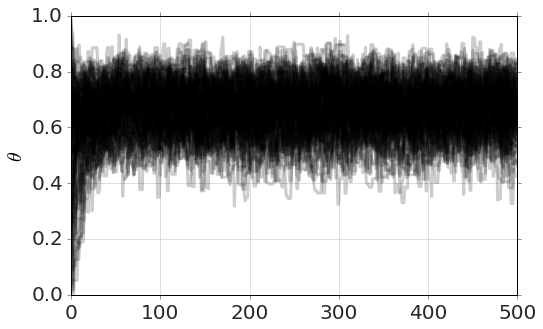
\includegraphics{output_6_2.png}
\caption{png}
\end{figure}

\subsubsection{run a bit longer\ldots{}}\label{run-a-bit-longer}

\begin{Shaded}
\begin{Highlighting}[]
\NormalTok{model.run_mcmc(}\DecValTok{500}\NormalTok{)}
\NormalTok{model.plot_chains()}
\end{Highlighting}
\end{Shaded}

\begin{verbatim}
Running MCMC...
Done.
0.78 s



<matplotlib.figure.Figure at 0x10e696e50>
\end{verbatim}

\begin{figure}[htbp]
\centering
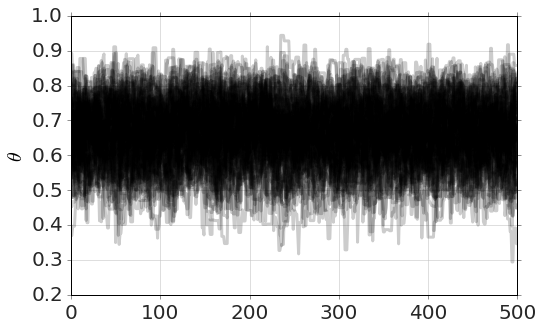
\includegraphics{output_8_2.png}
\caption{png}
\end{figure}

\subsubsection{\texorpdfstring{Plot the MCMC distribution of \(\theta\)
and the Beta distribution
solution}{Plot the MCMC distribution of \textbackslash{}theta and the Beta distribution solution}}\label{plot-the-mcmc-distribution-of-theta-and-the-beta-distribution-solution}

Hint: they should be the same

\begin{Shaded}
\begin{Highlighting}[]
\NormalTok{model.plot_distributions()}

\NormalTok{dist=coinflip(h,N)}
\NormalTok{x=linspace(}\DecValTok{0}\NormalTok{,}\FloatTok{1.0}\NormalTok{,}\DecValTok{100}\NormalTok{)}
\NormalTok{px=dist.pdf(x)}
\NormalTok{plot(x,px,}\StringTok{'r-'}\NormalTok{)}
\end{Highlighting}
\end{Shaded}

\begin{verbatim}
[<matplotlib.lines.Line2D at 0x10b78db90>]
\end{verbatim}

\begin{figure}[htbp]
\centering
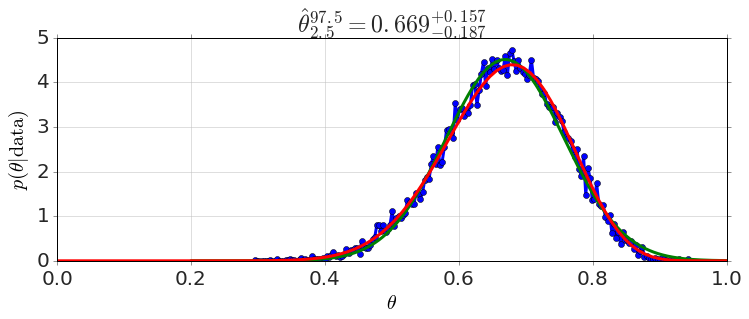
\includegraphics{output_10_1.png}
\caption{png}
\end{figure}

\subsubsection{Look at some
probabilitiess}\label{look-at-some-probabilitiess}

\begin{Shaded}
\begin{Highlighting}[]
\NormalTok{model.P(}\StringTok{'theta>0.5'}\NormalTok{)}
\end{Highlighting}
\end{Shaded}

\begin{verbatim}
0.96173333333333333
\end{verbatim}

\begin{Shaded}
\begin{Highlighting}[]
\NormalTok{model.P(}\StringTok{'(0.2<theta) & (theta<.5)'}\NormalTok{)}
\end{Highlighting}
\end{Shaded}

\begin{verbatim}
0.038266666666666664
\end{verbatim}

\subsection{Regression Example}\label{regression-example}

\begin{Shaded}
\begin{Highlighting}[]
\NormalTok{N=}\DecValTok{1000}
\NormalTok{x=arange(N)/}\FloatTok{1000.0}
\NormalTok{y=randn(N)+}\DecValTok{40}\FloatTok{+.25}\NormalTok{*x}
\NormalTok{plot(x,y,}\StringTok{'o'}\NormalTok{)}
\end{Highlighting}
\end{Shaded}

\begin{verbatim}
[<matplotlib.lines.Line2D at 0x110f7b410>]
\end{verbatim}

\begin{figure}[htbp]
\centering
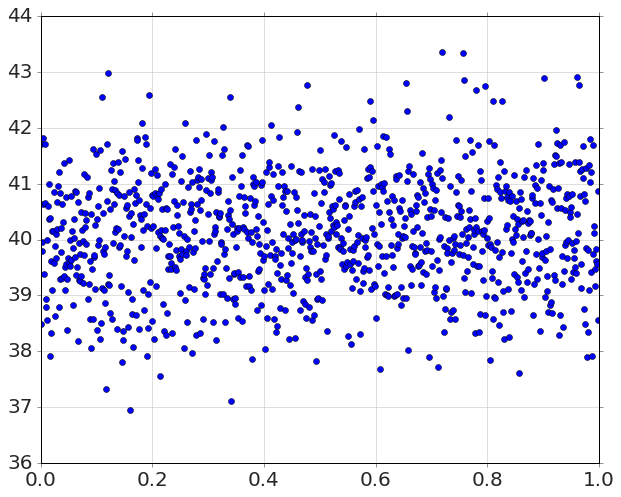
\includegraphics{output_15_1.png}
\caption{png}
\end{figure}

\begin{Shaded}
\begin{Highlighting}[]
\KeywordTok{def} \NormalTok{constant(x,a):}
    \KeywordTok{return} \NormalTok{a}

\NormalTok{model=MCMCModel_Regression(x,y,constant,}
            \NormalTok{a=Uniform(}\DecValTok{0}\NormalTok{,}\DecValTok{100}\NormalTok{),}
            \NormalTok{)}
\NormalTok{model.run_mcmc(}\DecValTok{500}\NormalTok{)}
\NormalTok{model.plot_chains()}
\end{Highlighting}
\end{Shaded}

\begin{verbatim}
Sampling Prior...
Done.
0.21 s
Running MCMC...
Done.
1.39 s



<matplotlib.figure.Figure at 0x10c028350>
\end{verbatim}

\begin{figure}[htbp]
\centering
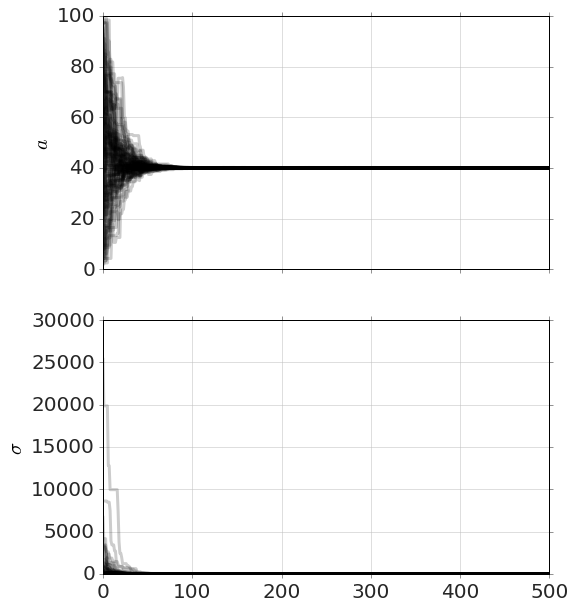
\includegraphics{output_16_2.png}
\caption{png}
\end{figure}

\begin{Shaded}
\begin{Highlighting}[]
\NormalTok{model.plot_distributions()}
\end{Highlighting}
\end{Shaded}

\begin{figure}[htbp]
\centering
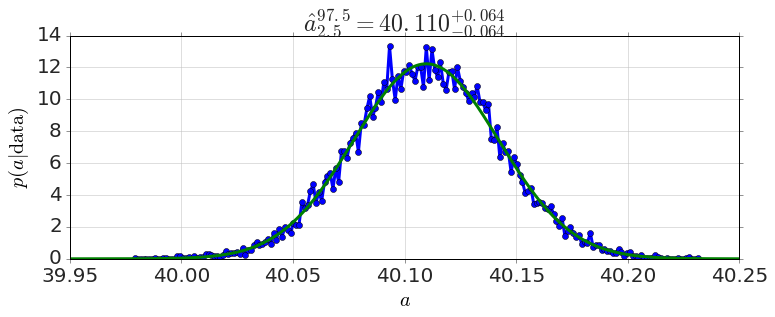
\includegraphics{output_17_0.png}
\caption{png}
\end{figure}

\begin{figure}[htbp]
\centering
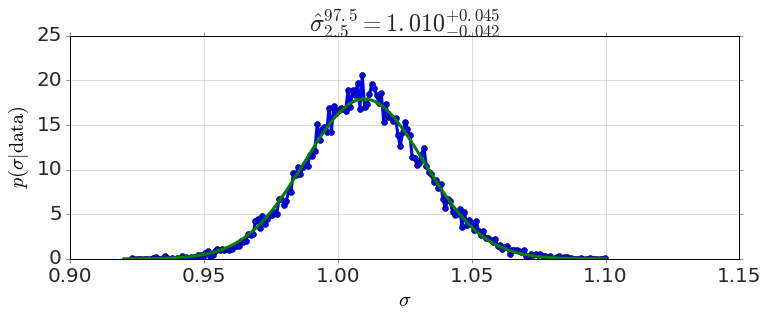
\includegraphics{output_17_1.png}
\caption{png}
\end{figure}

\begin{Shaded}
\begin{Highlighting}[]
\NormalTok{plot(x,y,}\StringTok{'o'}\NormalTok{)}

\NormalTok{xfit=linspace(}\DataTypeTok{min}\NormalTok{(x),}\DataTypeTok{max}\NormalTok{(x),}\DecValTok{200}\NormalTok{)}
\NormalTok{yfit=model.predict(xfit)}

\NormalTok{plot(xfit,yfit,}\StringTok{'-'}\NormalTok{)}
\end{Highlighting}
\end{Shaded}

\begin{verbatim}
[<matplotlib.lines.Line2D at 0x110f90c10>]
\end{verbatim}

\begin{figure}[htbp]
\centering
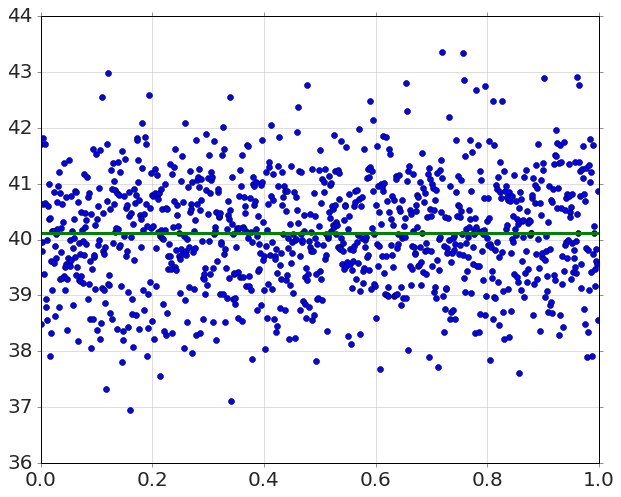
\includegraphics{output_18_1.png}
\caption{png}
\end{figure}

\begin{Shaded}
\begin{Highlighting}[]
\NormalTok{plot(x,y,}\StringTok{'o'}\NormalTok{)}
\NormalTok{model.plot_predictions(xfit,color=}\StringTok{'g'}\NormalTok{)}
\end{Highlighting}
\end{Shaded}

\begin{figure}[htbp]
\centering
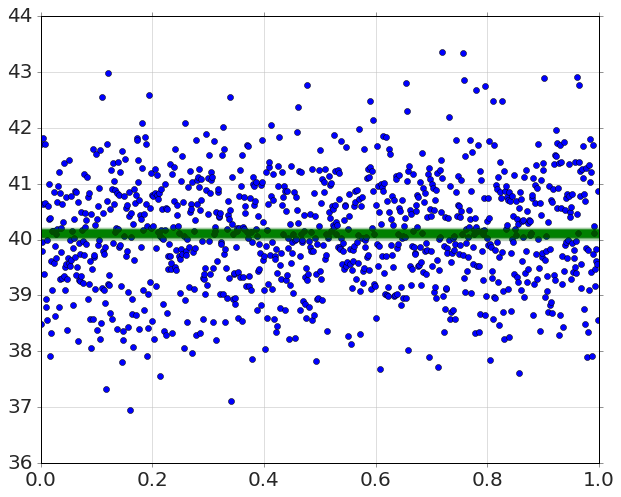
\includegraphics{output_19_0.png}
\caption{png}
\end{figure}

\subsection{Linear Model}\label{linear-model}

\begin{Shaded}
\begin{Highlighting}[]
\KeywordTok{def} \NormalTok{linear(x,a,b):}
    \KeywordTok{return} \NormalTok{a*x+b}

\NormalTok{model=MCMCModel_Regression(x,y,linear,}
                \NormalTok{a=Uniform(-}\DecValTok{10}\NormalTok{,}\DecValTok{10}\NormalTok{),}
                \NormalTok{b=Uniform(}\DecValTok{0}\NormalTok{,}\DecValTok{100}\NormalTok{),}
                \NormalTok{)}

\NormalTok{model.run_mcmc(}\DecValTok{500}\NormalTok{)}
\NormalTok{model.plot_chains()}
\end{Highlighting}
\end{Shaded}

\begin{verbatim}
Sampling Prior...
Done.
0.26 s
Running MCMC...
Done.
1.60 s



<matplotlib.figure.Figure at 0x11120bcd0>
\end{verbatim}

\begin{figure}[htbp]
\centering
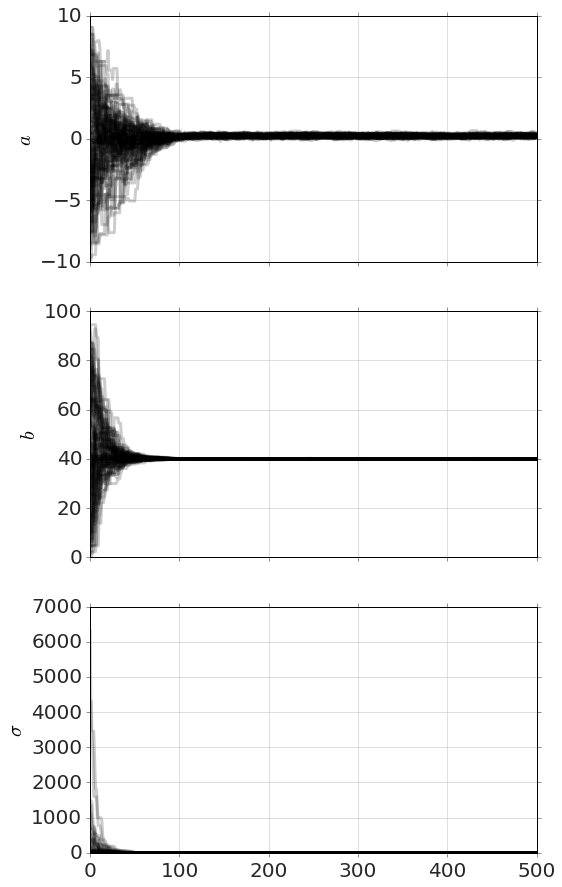
\includegraphics{output_21_2.png}
\caption{png}
\end{figure}

\begin{Shaded}
\begin{Highlighting}[]
\NormalTok{plot(x,y,}\StringTok{'o'}\NormalTok{)}
\NormalTok{model.plot_predictions(xfit,color=}\StringTok{'g'}\NormalTok{)}
\end{Highlighting}
\end{Shaded}

\begin{figure}[htbp]
\centering
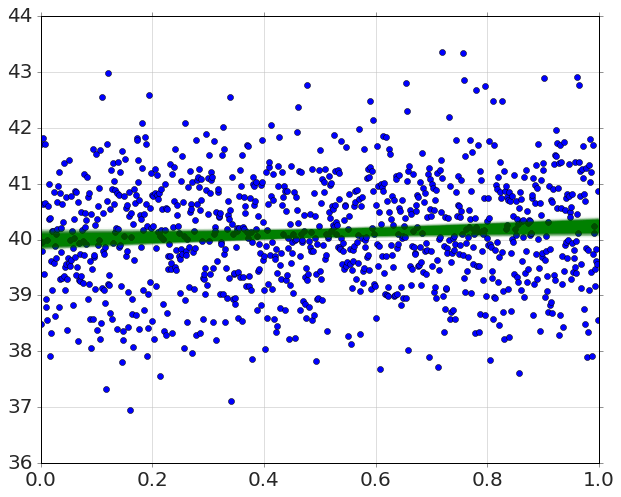
\includegraphics{output_22_0.png}
\caption{png}
\end{figure}

\begin{Shaded}
\begin{Highlighting}[]
\NormalTok{model.plot_distributions()}
\end{Highlighting}
\end{Shaded}

\begin{figure}[htbp]
\centering
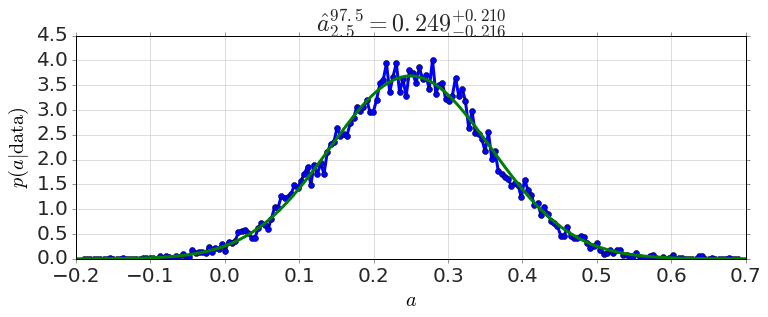
\includegraphics{output_23_0.png}
\caption{png}
\end{figure}

\begin{figure}[htbp]
\centering
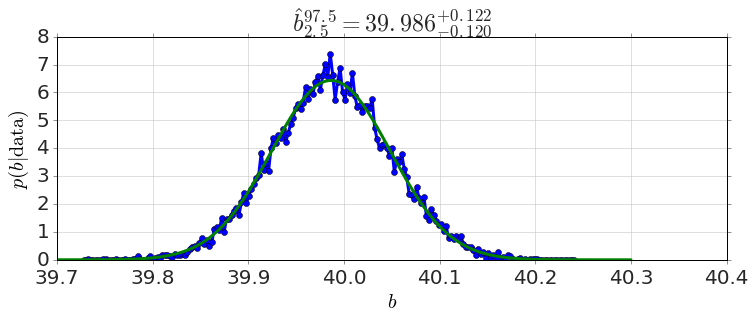
\includegraphics{output_23_1.png}
\caption{png}
\end{figure}

\begin{figure}[htbp]
\centering
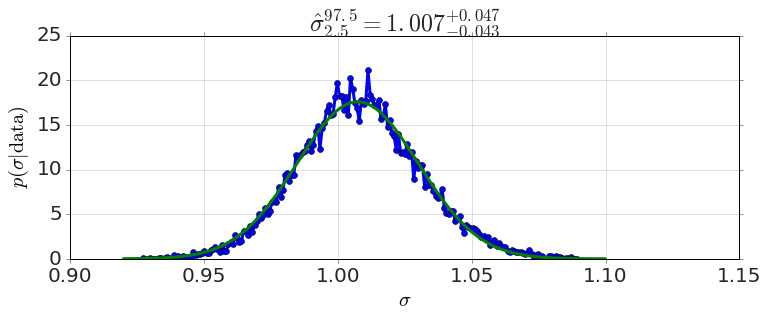
\includegraphics{output_23_2.png}
\caption{png}
\end{figure}

\begin{Shaded}
\begin{Highlighting}[]
\NormalTok{model.triangle_plot()}
\end{Highlighting}
\end{Shaded}

\begin{figure}[htbp]
\centering
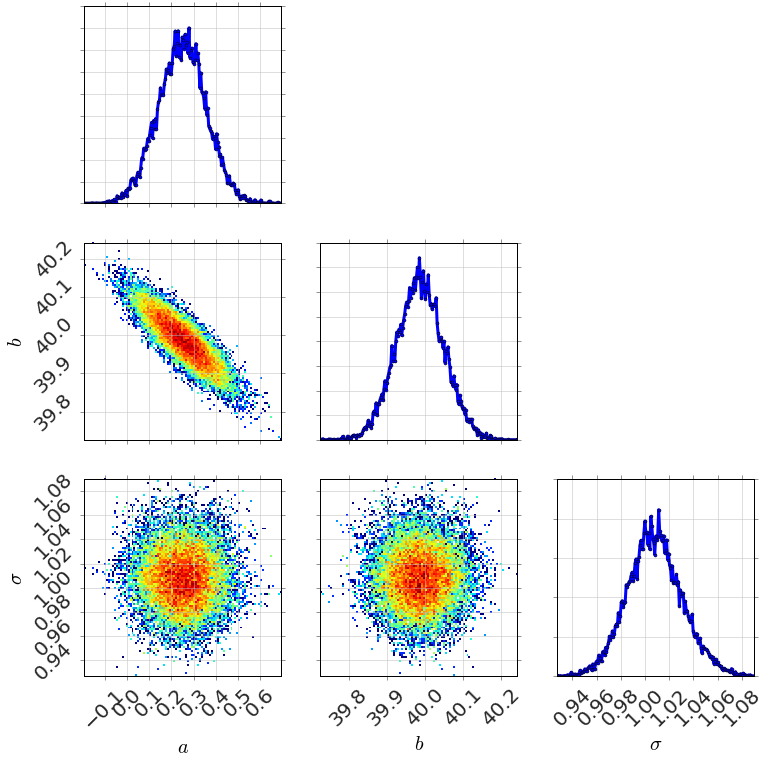
\includegraphics{output_24_0.png}
\caption{png}
\end{figure}

\begin{Shaded}
\begin{Highlighting}[]
\NormalTok{model.percentiles([}\DecValTok{5}\NormalTok{,}\DecValTok{50}\NormalTok{,}\DecValTok{95}\NormalTok{])}
\end{Highlighting}
\end{Shaded}

\begin{verbatim}
{'_sigma': array([ 0.97143798,  1.00744104,  1.0467333 ]),
 'a': array([ 0.07063144,  0.24939562,  0.42523751]),
 'b': array([ 39.88446461,  39.98633744,  40.09010139])}
\end{verbatim}

\begin{Shaded}
\begin{Highlighting}[]
\NormalTok{model.P(}\StringTok{'a>0'}\NormalTok{)}
\end{Highlighting}
\end{Shaded}

\begin{verbatim}
0.98936000000000002
\end{verbatim}

\begin{Shaded}
\begin{Highlighting}[]

\end{Highlighting}
\end{Shaded}

\end{document}